%%% Appendix %%%
\section{Hyperparameters}
\unskip\label{sec:hparams}

\subsection{Causal language modeling}
\unskip\label{sec:hparams-clm}

For values not listed, see Hugging Face Transformers' defaults at \url{https://huggingface.co/docs/transformers/v4.36.1/en//model_doc/gpt2\#transformers.GPT2Config}.
\begin{itemize}[itemsep=-1.2ex]
  \item Model: GPT-2
  \item Tokenizer: Byte pair encoding
  \item Hidden size: $768$ (default)
  \item Vocabulary size: $30\,000$
  \item Context length: $256$
  \item Number of layers: $6$
  \item Number of attention heads: $6$
  \item Learning rate: $1\cdot10^{-4}$
  \item Optimizer: AdamW
  \item Weight decay: $0.01$
  \item Learning rate schedule: linear (to $0$)
  \item Batch size: $32$
  \item Train dataset size: $15\cdot10^6$ tokens
  \item Train epochs: $5$
  \item Tune dataset size: $2\cdot10^6$ tokens
  \item Train epochs: $10$
\end{itemize}


\subsection{Machine translation}
\unskip\label{sec:hparams-mt}
For values not listed, see Hugging Face Transformers' defaults at \url{https://huggingface.co/docs/transformers/v4.36.1/en/model_doc/bart\#transformers.BartConfig}.
The following is for the \emph{Full} setting.
\begin{itemize}[itemsep=-1.2ex]
  \item Model: BART
  \item Training objective: text infilling only (see note below)
  \item Tokenizer: Byte pair encoding
  \item Hidden size: $512$
  \item Vocabulary size: $30\,000$
  \item Context length: $512$
  \item Number of encoder layers: $6$
  \item Number of decoder layers: $6$
  \item Number of encoder attention heads: $8$
  \item Number of decoder attention heads: $8$
  \item Encoder feedforward dimension: $2048$
  \item Decoder feedforward dimension: $2048$
  \item Train learning rate: $1\cdot10^{-4}$
  \item Tune learning rate: $2\cdot10^{-4}$
  \item Optimizer: AdamW
  \item Weight decay: $0.01$
  \item Learning rate schedule: linear (to $0$)
  \item Batch size: $32$
  \item Train dataset size: $100\cdot10^6$ tokens
  \item Train epochs: $5$
  \item Tune dataset size: $50\cdot10^6$ tokens
  \item Train epochs: $3$
  \item Test beam size: $1,3,5$ (final metric averaged across each size)
  \item Test context size: $128$
\end{itemize}
The objective used to pretrain BART was text infilling \emph{only}; we cannot use the sentence permutation objective because we do not know \emph{a priori} what constitutes a sentence in an emergent language, hence we do not use it for any settings.
For the \emph{Frozen} setting, all is as above, but all non-embedding layers are frozen for the duration of tuning.
For the \emph{Reduced} setting, all is as above except for the following:
\begin{itemize}[itemsep=-1.2ex]
  \item Tune learning rate: $1\cdot10^{-5}$
  \item Tune dataset size: $10\cdot10^6$
\end{itemize}

\subsection{Generic signalling game}
\unskip\label{sec:hparams-egg}
We use the following hyperparameters for the \emph{Disc, small} emergent language.
\begin{itemize}[itemsep=-1.2ex]
  \item Game (from EGG): \\\texttt{egg.zoo.basic\_games.play}
  \item Message optimization: Gumbel-softmax (as opposed to REINFORCE)
  \item Game type: discrimination
  \item Number of attributes: $4$
  \item Number of values: $4$
  \item Number of distractors: $5$
  \item Vocabulary size: $6$
  \item Max message length: $10$
  \item Number of examples: $32\,768$
  \item Batch size; $1024$
  \item Number of epochs: $10$
  \item Sender hidden size: $256$
  \item Receiver hidden size: $512$
  \item Sender embedding size: $32$
  \item Receiver embedding size: $32$
  \item Sender network type: GRU
  \item Receiver network type: GRU
  \item Learning rate: $0.001$
\end{itemize}
The \emph{Disc, large} setting uses the same hyperparameters as above with the exception of the following.
\begin{itemize}[itemsep=-1.2ex]
  \item Number of attributes: $12$
  \item Number of values: $8$
  \item Number of distractors: $5$
  \item Number of examples: $3.5\cdot10^6$
  \item Max message length: $30$
  \item Vocabulary size: $100$
  \item Number of epochs: $100$
\end{itemize}
The \emph{Recon, large} setting is as in \emph{Disc, large} with the following changes.
\begin{itemize}[itemsep=-1.2ex]
  \item Game type: reconstruction
  \item Number of attributes: $8$
  \item Number of distractors: N/A
  \item Number of examples: $1\cdot10^6$
  \item Number of epochs: $10$
\end{itemize}


\section{Example of benchmark input format}
\unskip\label{sec:input-example}

The input format for the benchmark is simple: integer arrays in a JSON format separated by newlines (i.e., JSON Lines, JSONL, {\small\texttt{{}*.jsonl}}).
The following is an example of file contents in this format:
\begin{verbatim}
[3, 1, 4, 1, 5, 9, 2]
[6, 5, 3, 5, 8, 9, 7, 9, 3]
[2, 3, 8, 4]
[6, 2, 6, 4, 3, 3]
[8, 3, 2, 7, 9, 5, 0, 2, 8, 8, 4]
\end{verbatim}



\section{Computing resources used}
See \Cref{tab:compute} for rough estimates of the compute used in writing this paper.
Most experiments were run on a shared cluster comprising approximately $150$ NVIDIA A6000 (or comparable) GPUs.
\begin{table}
  \centering
  \begin{tabular}{lrrr}
    \toprule
    Item & Base GH & $n$ items & Total \\
    \midrule
    XferBench         & $6$ & $45$ & $270$ \\
    MT                & $8$ & $50$ & $400$ \\
    Other experiments & $2$ & $50$ & $100$ \\
    \midrule
    Total             & & & $770$ \\
    \bottomrule
  \end{tabular}
  \caption{Estimate of compute used for this paper in GPU-hours (specifically NVIDIA RTX 2080 Ti--hours).}
  \unskip\label{tab:compute}
\end{table}


\section{Additional results}

\subsection{BLEU scores for machine translation}
\unskip\label{sec:mt-bleu}
See \Cref{tab:mt-bleu}.
\begin{table}
  \centering
  \inputsrc{figures/mt-bleu}
  \caption{BLEU scores for machine translation experiment.  Colors normalized by column.}
  \unskip\label{tab:mt-bleu}
\end{table}

\subsection{Raw cross-entropies on XferBench}
\unskip\label{sec:clm-all}
See \Cref{tab:clm-all}.
\begin{table*}
  \centering
  \inputsrc{figures/clm-all}
  \caption{Cross-entropies across all source and target languages. Colors normalized by column.}
  \unskip\label{tab:clm-all}
\end{table*}

\subsection{Writing system matrix for normalized XferBench scores}
\unskip\label{sec:clm-writing-system}

See \Cref{tab:clm-writing-system,tab:clm-writing-system-type}.
Scores for reach writing system are aggregated by taking the mean.
\Cref{tab:writing-system} gives the writing system classification for the languages used in the experiments.
Although the class imbalance makes it impossible to draw any definitive claims, the preliminary results do not suggest any correlation in XferBench between the writing systems of the source and target languages.

% "fr": ("Latin", "Alphabet"),
% "es": ("Latin", "Alphabet"),
% "ru": ("Cyrillic", "Alphabet"),
% "zh": ("Chinese", "Logographic"),
% "ko": ("Hangul", "Alphabet"),
% "ar": ("Arabic", "Abjad"),
% "hi": ("Devanagari", "Aguida"),
% "da": ("Latin", "Alphabet"),
% "eu": ("Latin", "Alphabet"),
% "fa": ("Arabic", "Abjad"),
% "fi": ("Latin", "Alphabet"),
% "he": ("Hebrew", "Abjad"),
% "id": ("Latin", "Alphabet"),
% "ja": ("Japanese", "Mixed"),
% "kk": ("Cyrillic", "Alphabet"),
% "ro": ("Latin", "Alphabet"),
% "ur": ("Arabic", "Abjad"),

\begin{table}
  \centering
  \begin{tabular}{lll}
    \toprule
    Type & Writing System & Language \\
    \midrule
    \multirow{4}{*}{Abjad} & \multirow{3}{*}{Arabic} & ar \\
            & & fa \\
            & & ur \\
        \cmidrule{2-3}
        & Hebrew & he \\
        \midrule
    Abugida & Devanagari & hi \\
    \midrule
    \multirow{10}{*}{Alphabet} & \multirow{2}{*}{Cyrillic} & kk \\
            & & ru \\
        \cmidrule{2-3}
        & Hangul & ko \\
        \cmidrule{2-3}
        & \multirow{7}{*}{Latin} & da \\
            & & es \\
            & & eu \\
            & & fi \\
            & & fr \\
            & & id \\
            & & ro \\
    \midrule
    Logographic & Chinese & zh \\
    \midrule
    Mixed & Japanese & ja \\
    \bottomrule
  \end{tabular}
  \caption{%
    Coarse and fine classifications of writing systems of human languages (source and target) used in the experiments.
  }
  \unskip\label{tab:writing-system}
\end{table}


\begin{table*}
  \centering
  \inputsrc{figures/clm-writing-system}
  \caption{%
    Normalized XferBench scores by writing system (lower is better).
    Color is normalized across all values.
  }
  \unskip\label{tab:clm-writing-system}
\end{table*}

\begin{table*}
  \centering
  \inputsrc{figures/clm-writing-system-type}
  \caption{%
    Normalized XferBench scores by writing system type (lower is better).
    Color is normalized across all values.
  }
  \unskip\label{tab:clm-writing-system-type}
\end{table*}

\subsection{Scatter plots for XferBench and MT}
\unskip\label{sec:scatter}
See \Cref{fig:scatter}.
\begin{figure*}
  \centering
  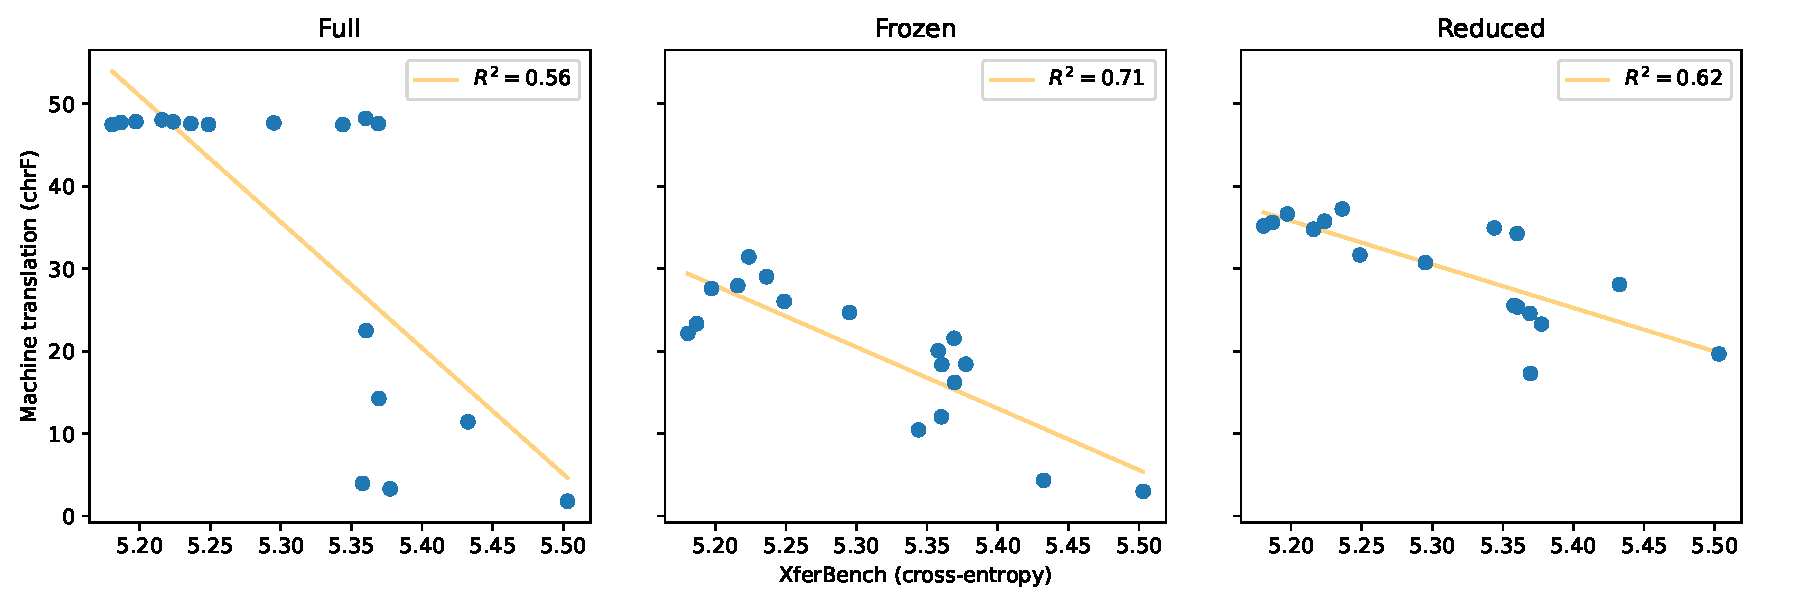
\includegraphics[width=\textwidth]{chapters/xferbench/src/figures/correlation}
  \caption{Scatter plots showing XferBench score versus machine translation score.}
  \unskip\label{fig:scatter}
\end{figure*}

\section{Cross-entropy confidence interval computation}
\unskip\label{sec:bootstrapping}

Let $s \in S$ and $t \in T$ represent source and target languages, respectively.
$h_{s,t}$ represents the test cross-entropy of a model pretrained on $s$ and evaluated on $t$.
As sated in \Cref{eq:hs}, the score on XferBench is the mean cross-entropy across all target languages:
\begin{align}
  h_{s} &= \mean_{t' \in T}\left( h_{s,t'}\right)
  .
\end{align}
We would like to calculate a confidence interval (i.e., $h^-_s$ and $h^+_s$) for a source language's mean cross-entropy using the different cross-entropies on the target languages (i.e., $h_{s,t}$ for $t \in T$), yet these samples are not i.i.d., since the mean of cross-entropy each \emph{target} language can vary.
Thus, if we would like to use bootstrapping to calculate confidence intervals, we must first normalize the cross-entropies.
Let $\hat h_{s,t}$ be the normalized score:
\begin{align}
  \hat h_{s,t} &= \frac{h_{s,t} - \mean_{s'\in S}\left(h_{s',t}\right)}{\stdev_{s'\in S}\left(h_{s',t}\right)}
  .
\end{align}
Given the normalized scores, we can now bootstrap in order to compute confidence intervals for $\hat h_s$ (i.e., in the normalized space).\footnote{This is not intended to be statistically rigorous. Our cross-entropies are unlikely to be normally distributed, but this still be helpful for generally gauging uncertainty.}
Let $\hat h^+_s$ and $\hat h^-_s$ be the upper and lower bounds of the confidence interval computed using bootstrapping in the normalized space.
We can now translate these back into the raw cross-entropy space using the means and standard deviations from before:
\begin{align}
  h^+_s &= \hat h^+_s \cdot \stdev_{s'\in S}\left(h_{s',t}\right) + \mean_{s'\in S}\left(h_{s',t}\right) \\
  h^-_s &= \hat h^-_s \cdot \stdev_{s'\in S}\left(h_{s',t}\right) + \mean_{s'\in S}\left(h_{s',t}\right)
  .
\end{align}

\section{Error analysis}
\unskip\label{sec:error-analysis}
In the \emph{Full} setting of the machine translation task, the \emph{Yao+} and \emph{Mu+, SW} settings perform worse than expected (\emph{a priori} and compared to the other results in the setting).
Validation loss converged while chrF and BLEU scores remained near zero.
We provide a couple examples (taken from the predefined test set of WMT 2014) of model output to provide some insight into the reason for this.
No post processing used, generation is capped at $50$ tokens, and ``\textbackslash{}u0000'' represent single non-printable characters.

\paragraph{Example 1}
\emph{Input}: ``And while Congress can't agree on whether to proceed, several states are not waiting.''

\emph{Reference}: ``Et tandis que les membres du Congrès n'arrivent pas à se mettre d'accord pour savoir s'il faut continuer, plusieurs États n'ont pas attendu.''

[Model pretrained on] \emph{French}:
``\#Et alors que le Congrès ne peut pas convenir de poursuivre, plusieurs États ne sont pas en attente. » (traduction libre) Le Parlement européen. Le Parlement européen est d’avis que le Parlement européen doit être en mesure de faire preuve\#''

\emph{Disc, large}:
``\#Et bien que le Congrès ne puisse pas convenir de la marche à suivre, plusieurs États ne sont pas en attente.\textbackslash{}u2028\textbackslash{}u2028[Traduit par la Rédaction]\textbackslash{}u2028(Traduit par la Rédaction)\textbackslash{}u2028(Tra\#''

\emph{Yao+}:
``\#Annexe II, par.\allowbreak{}\textbackslash{}xa02.\allowbreak{}2.\allowbreak{}2.\allowbreak{}2.\allowbreak{}2.\allowbreak{}2.\allowbreak{}2.\allowbreak{}2.\allowbreak{}2.\allowbreak{}2.\allowbreak{}2.\allowbreak{}2.\allowbreak{}2.\allowbreak{}2.\allowbreak{}2.\allowbreak{}2.\allowbreak{}2.\allowbreak{}2.\allowbreak{}2.\allowbreak{}2.\allowbreak{}2.\allowbreak{}\#''

\emph{Mu+, SW}:
``\#Annexe II.\allowbreak{}\textbackslash{}xa0\allowbreak{}\textbackslash{}xa0: Appendice I.\allowbreak{}\textbackslash{}xa0I.\allowbreak{}\textbackslash{}xa0I.\allowbreak{}\textbackslash{}xa0I.\allowbreak{}\textbackslash{}xa0I.\allowbreak{}\textbackslash{}xa0I.\allowbreak{}\textbackslash{}xa0I.\allowbreak{}\textbackslash{}xa0I.\allowbreak{}\textbackslash{}xa0I.\allowbreak{}\textbackslash{}xa0I.\allowbreak{}\textbackslash{}xa0I.\allowbreak{}\textbackslash{}xa0I.\allowbreak{}\textbackslash{}xa0I.\allowbreak{}\textbackslash{}xa0I\#''

\paragraph{Example 2}
\emph{Input}:
``This really is a must for our nation.''

\emph{Reference}:
``Cela est vraiment indispensable pour notre nation.''

\emph{French}:
``\#C'est vraiment une nécessité pour notre nation. Nous devons y parvenir. Nous devons y parvenir. Nous devons y parvenir. Nous devons y parvenir. Nous devons y parvenir. Nous devons y parvenir. Nous devons y parvenir. Nous devons y\#''

\emph{Disc, large}:
``\#C'est vraiment un devoir pour notre nation. C'est un devoir.\textbackslash{}u2028\allowbreak{}\textbackslash{}u2028(...)\allowbreak{}\textbackslash{}u2028\allowbreak{}\textbackslash{}u2028(...)\allowbreak{}\textbackslash{}u2028(...)\allowbreak{}\textbackslash{}u2028(...)\allowbreak{}\textbackslash{}u2028(...)\allowbreak{}\textbackslash{}u2028(...)\allowbreak{}\textbackslash{}u2028(...)\allowbreak{}\textbackslash{}u2028(\#''

\emph{Yao+}:
``\#Annexe II, par.\allowbreak{}\textbackslash{}xa02.\allowbreak{}2.\allowbreak{}2.\allowbreak{}2.\allowbreak{}2.\allowbreak{}2.\allowbreak{}2.\allowbreak{}2.\allowbreak{}2.\allowbreak{}2.\allowbreak{}2.\allowbreak{}2.\allowbreak{}2.\allowbreak{}2.\allowbreak{}2.\allowbreak{}2.\allowbreak{}2.\allowbreak{}2.\allowbreak{}2.\allowbreak{}2.\allowbreak{}2.\allowbreak{}\#''

\emph{Mu+, SW}:
``\#Annexe II.\allowbreak{}\textbackslash{}xa0\allowbreak{}\textbackslash{}xa0: Appendice I.\allowbreak{}\textbackslash{}xa0I.\allowbreak{}\textbackslash{}xa0I.\allowbreak{}\textbackslash{}xa0I.\allowbreak{}\textbackslash{}xa0I.\allowbreak{}\textbackslash{}xa0I.\allowbreak{}\textbackslash{}xa0I.\allowbreak{}\textbackslash{}xa0I.\allowbreak{}\textbackslash{}xa0I.\allowbreak{}\textbackslash{}xa0I.\allowbreak{}\textbackslash{}xa0I.\allowbreak{}\textbackslash{}xa0I.\allowbreak{}\textbackslash{}xa0I.\allowbreak{}\textbackslash{}xa0I\#''

\paragraph{Discussion}
Although all of the models have trouble terminating properly, the \emph{French} and \emph{Disc, large} models (which have high chrF scores) clearly condition their generation on the text, whereas \emph{Yao+} and \emph{Mu+, SW} give the same output regardless of the input.
Although this is unexpected, we can see in the \emph{Full} setting in \Cref{fig:scatter} that there is sharp drop off between high-performing and low-performing languages.
We suspect that the higher learning rate during tuning caused this bimodal distribution of results and is at least in part responsible for the poor performance \emph{Yao+} and \emph{Mu+, SW} models on the MT experiment's \emph{Full} setting.



\typeout{INFO: \arabic{comment} comments.}
